\documentclass[conference]{IEEEtran}
\IEEEoverridecommandlockouts
\usepackage{cite}
\usepackage{amsmath,amssymb,amsfonts}
\usepackage{algorithmic}
\usepackage{graphicx}
\graphicspath{ {./lineplot/} }
\usepackage{textcomp}
\usepackage{hyperref}
\usepackage{xcolor}
% code shannigans
\usepackage{listings}
\usepackage{color}

\definecolor{dkgreen}{rgb}{0,0.6,0}
\definecolor{gray}{rgb}{0.5,0.5,0.5}
\definecolor{mauve}{rgb}{0.58,0,0.82}

\lstset{frame=tb,
  language=Java,
  aboveskip=3mm,
  belowskip=3mm,
  showstringspaces=false,
  columns=flexible,
  basicstyle={\small\ttfamily},
  numbers=none,
  numberstyle=\tiny\color{gray},
  keywordstyle=\color{blue},
  commentstyle=\color{dkgreen},
  stringstyle=\color{mauve},
  breaklines=true,
  breakatwhitespace=true,
  tabsize=3
}

% code shannigans end

\def\BibTeX{{\rm B\kern-.05em{\sc i\kern-.025em b}\kern-.08em
T\kern-.1667em\lower.7ex\hbox{E}\kern-.125emX}}
\begin{document}

\title{Popularity of Programming languages over the years\\
{\footnotesize \textsuperscript{}Data analysis on most popular programming languages from 2004 to 2022}}


\author{\IEEEauthorblockN{Aryan Singh}
\IEEEauthorblockA{\textit{Department of Computer Science and Engineering} \\
\textit{Meghnad Saha Institute of Technology}\\
Calcutta, India \\
\texttt{aryansingh\_cse2021@msit.edu.in}}
\and
\IEEEauthorblockN{Neeraj P Pillai}
\IEEEauthorblockA{\textit{Department of Computer Science and Engineering} \\
\textit{Meghnad Saha Institute of Technology}\\
Calcutta, India \\
\texttt{neeraj\_p.cse2021@msit.edu.in}}
\and
\IEEEauthorblockN{Abdul Basit}
\IEEEauthorblockA{\textit{Department of Computer Science and Engineering} \\
\textit{Meghnad Saha Institute of Technology}\\
Calcutta, India \\
\texttt{abdul\_b.cse2021@msit.edu.in}}
\and
\IEEEauthorblockN{Kuntal Barik}
\IEEEauthorblockA{\textit{Department of Computer Science and Engineering} \\
\textit{Meghnad Saha Institute of Technology}\\
Calcutta, India \\
\texttt{kuntal\_b.cse2021@msit.edu.in}}
\and
\IEEEauthorblockN{Harshil D Sheth}
\IEEEauthorblockA{\textit{Department of Computer Science and Engineering} \\
\textit{Meghnad Saha Institute of Technology}\\
Calcutta, India \\
\texttt{hdsheth.cse2021@msit.edu.in}}
}

\maketitle

\begin{abstract}
We begin with the age-old and divisive question "Which is the best programming language?". But with a willingness to keep the same number of friends, when we started out with this project!
\end{abstract}

\section{Introduction}
This project is based on data analysis of popular programming languages over the decades
We have used the functionality provided by the Python programming language and libraries built for the same. The libraries used are Pandas, Numpy, and Seaborn. The data collected has been categorically sorted into months leading to January 2022. In this project, we have discussed how languages have held up over the years.

\subsection{Primary Categorisation}\label{AA}
We have settled into four primary categorisations : 

\begin{itemize}
\item \textbf{[PP]} The languages which have remained popular over the years.
\item \textbf{[PF]} The languages which are no longer popular.
\item \textbf{[FP]} The languages which have become popular.
\item \textbf{[FF]} Languages that never gained market dominance.
\end{itemize}

\subsection{Secondary Categorisation}
The secondary category are designed to include languages that show  trends that do not necessarily fit into what we have established in the primary categories, secondary categories :
\begin{itemize}
\item "Mid for Life", this category has been named after a popular gen-z slang ''mid'' meaning below average.
\item "Gaining Popularity", this category includes languages that are early in development and are gaining market rapidly.
\end{itemize}

\section{Definitions}
\textbf{Popular:} for a language to be considered popular a minimum of 8% or 8 out of every 100 people must use the language. 

\textbf{Mid:} is a language that never crossed the upper boundary of 7% and a lower boundary of 3%.

\textbf{Bust:} is a language that never gained more than 3% of the dominant market share.

\section{Primary Classification}

\subsection{PP}
The languages which have remained popular over the year. The only language in our data-set that fits with this description of ours is JavaScript.
\begin{itemize}
\item{Javacript}
\end{itemize}

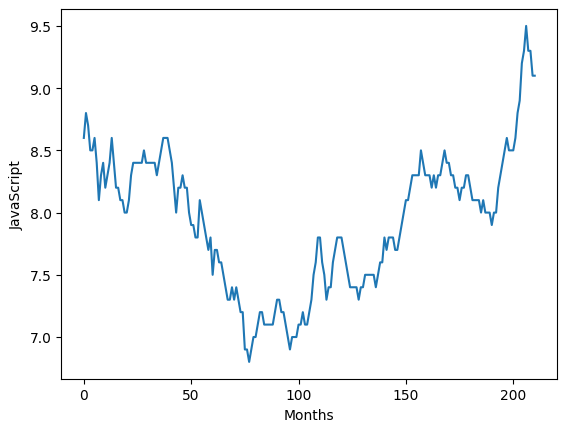
\includegraphics[scale=0.4]{lineplot/javascript.png}


\subsection{PF}
The languages which are no longer popular.

\begin{itemize}
\item{Visual Basic}
\item{PHP}:Although PHP never reached a market dominant position, reaching a maximum position of \(20.8%\) market share we can however correlate its downfall to Python with a correlation coefficient of \(-0.943219\)
\item{Perl}
\item{Java}
\end{itemize}

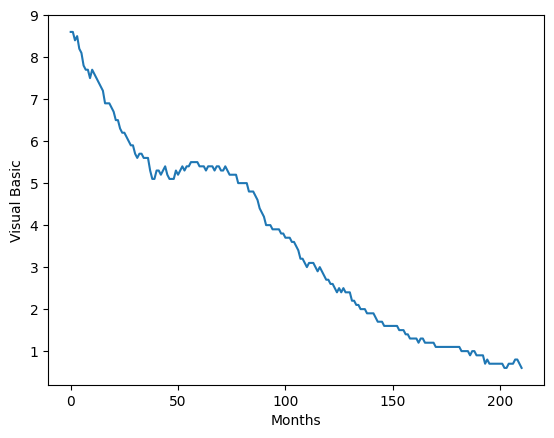
\includegraphics[scale=0.4]{lineplot/visualbasic.png}
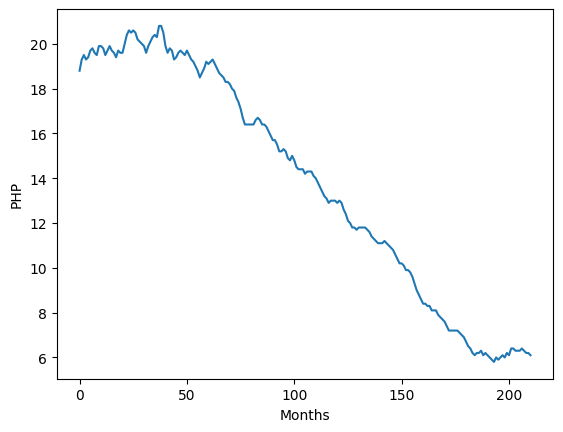
\includegraphics[scale=0.4]{lineplot/php.png}
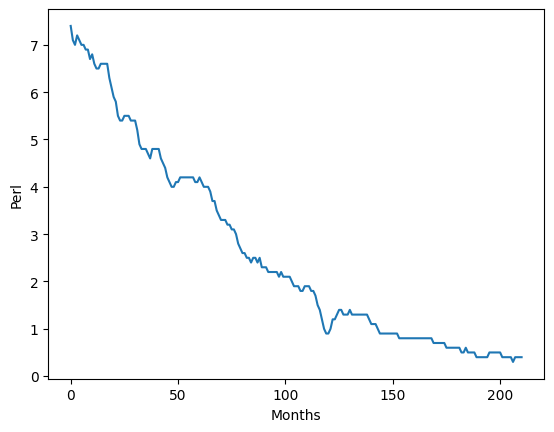
\includegraphics[scale=0.4]{lineplot/perl.png}
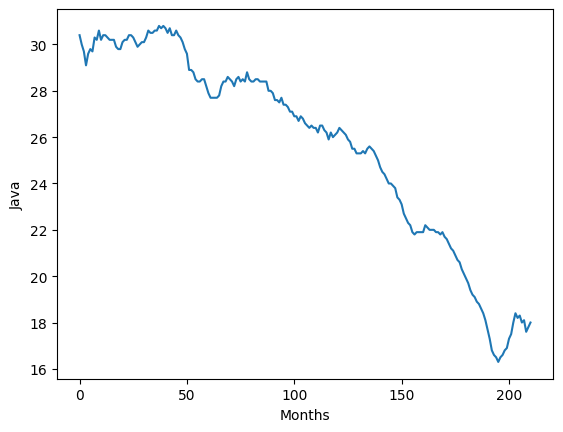
\includegraphics[scale=0.4]{lineplot/java.png}

\subsection{FP}
The languages which have become popular. The only language fitting this description of ours is Python.
\begin{itemize}
\item{Python}
\end{itemize}

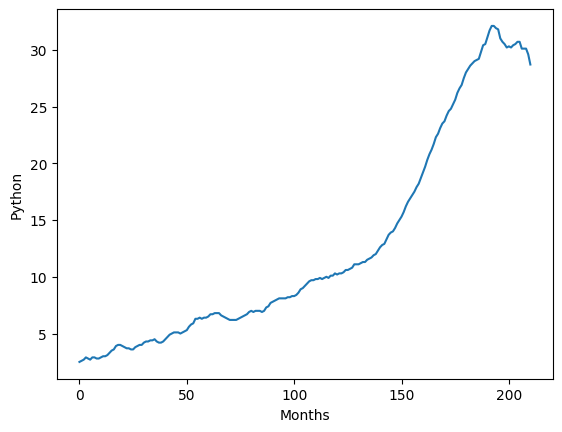
\includegraphics[scale=0.4]{lineplot/python.png}

\subsection{FF}
The languages that never gained market dominance

\begin{itemize}
\item{VBA}
\item{Scala}
\item{Rust}
\item{Lua}
\item{Pascal}
\item{Cobol}
\item{Ada}
\item{Abap}
\end{itemize}

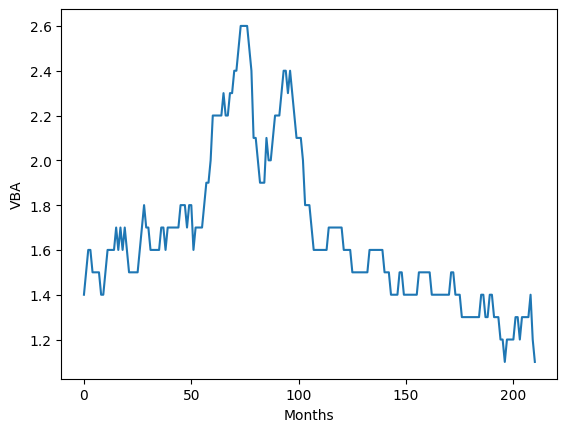
\includegraphics[scale=0.4]{lineplot/vba.png}
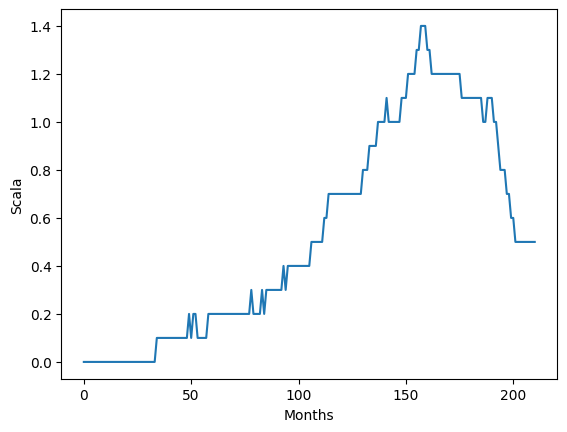
\includegraphics[scale=0.4]{lineplot/scala.png}
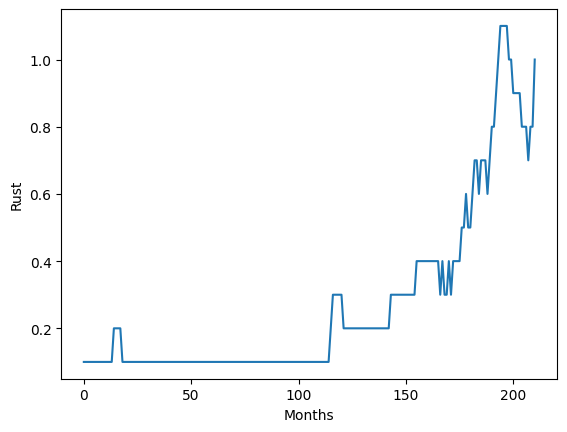
\includegraphics[scale=0.4]{lineplot/rust.png}
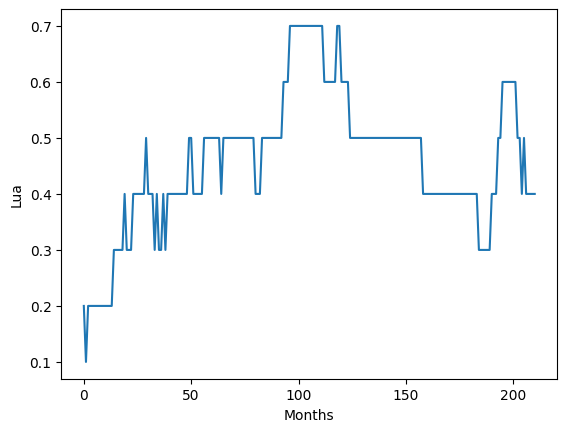
\includegraphics[scale=0.4]{lineplot/lua.png}
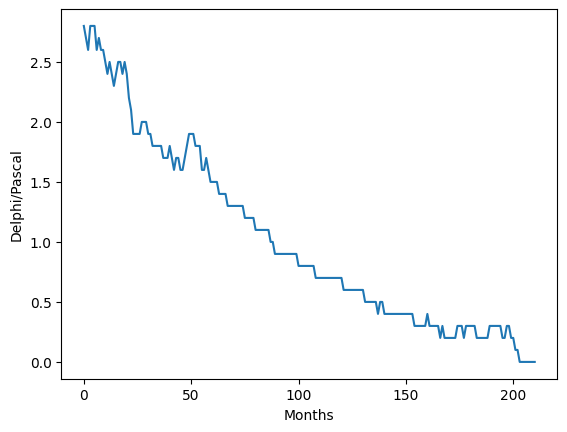
\includegraphics[scale=0.4]{lineplot/pascal.png}
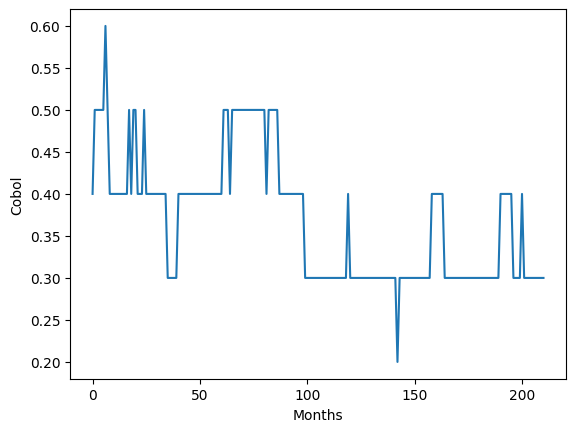
\includegraphics[scale=0.4]{lineplot/cobol.png}
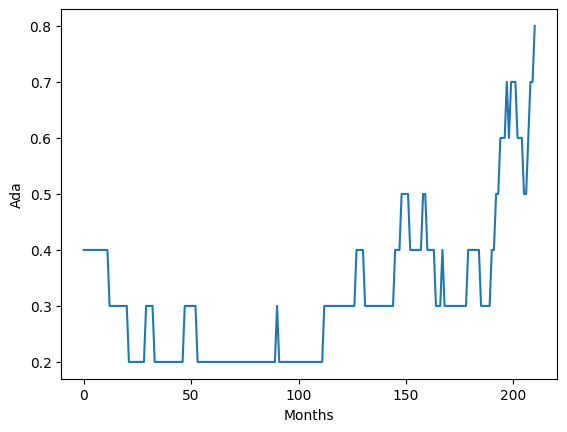
\includegraphics[scale=0.4]{lineplot/ada.png}
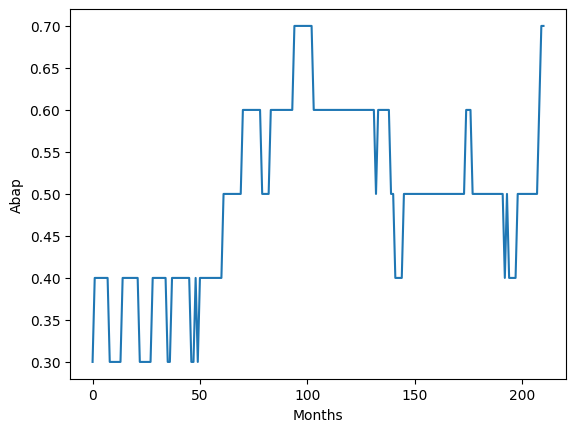
\includegraphics[scale=0.4]{lineplot/abap.png}

\section{Secondary Classification}

\subsection{\textit{Mid for life}}
This category has been named after a popular gen-z slang ''mid'' meaning below average.
These languages have been included in this category not because they are haphazardly engineered but because they were created for a specific purpose and their development cycle highlights and emphasizes their original purposes. For example C Sharp (C#) was created for game development and it is still a cult classic.

\begin{itemize}
\item{Swift}
\item{Ruby}
\item{Objective-C}
\item{Matlab}
\item{Kotlin}
\item{Julia}
\item{Haskell}
\item{C sharp}
\item{C/C++}
\end{itemize}

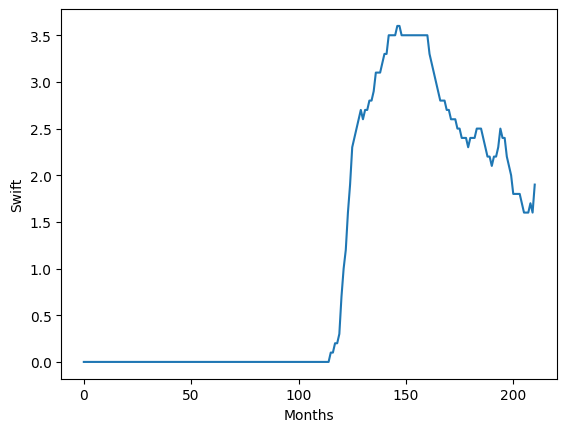
\includegraphics[scale=0.4]{lineplot/swift.png}
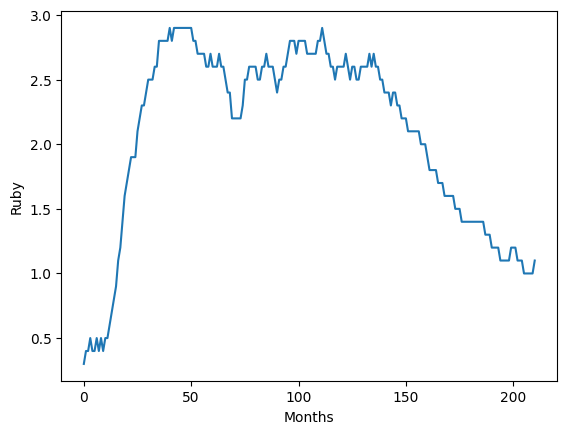
\includegraphics[scale=0.4]{lineplot/ruby.png}
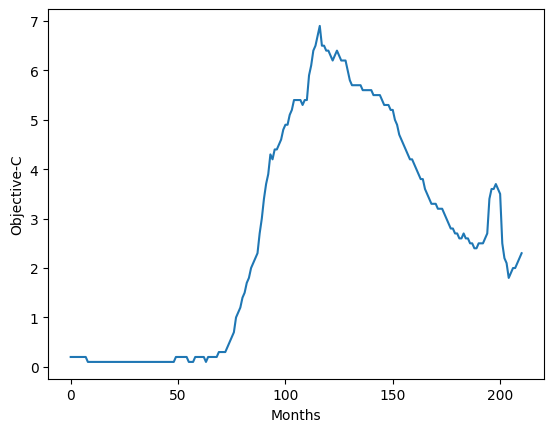
\includegraphics[scale=0.4]{lineplot/objective-c.png}
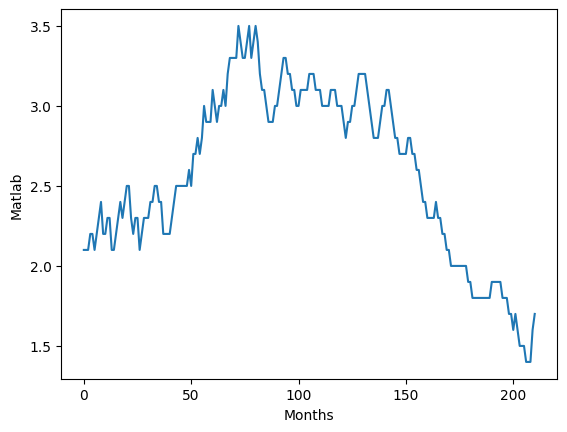
\includegraphics[scale=0.4]{lineplot/matlab.png}
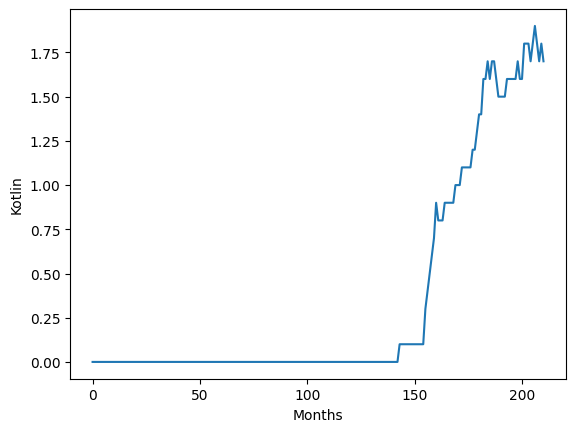
\includegraphics[scale=0.4]{lineplot/kotlin.png}
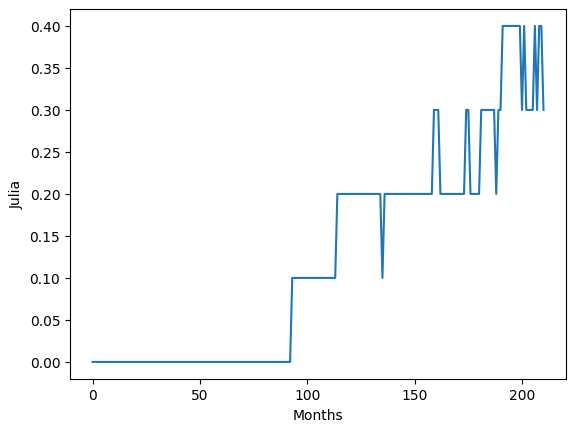
\includegraphics[scale=0.4]{lineplot/julia.png}
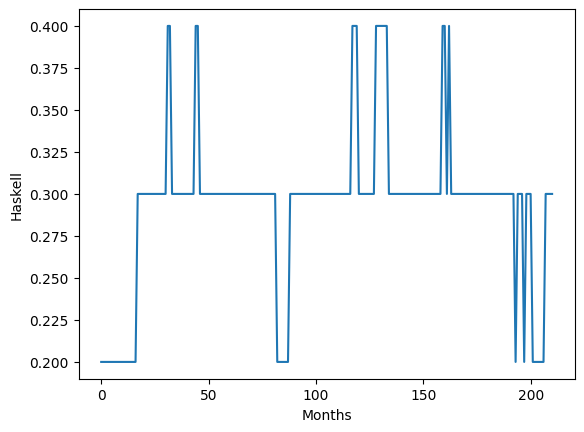
\includegraphics[scale=0.4]{lineplot/haskell.png}
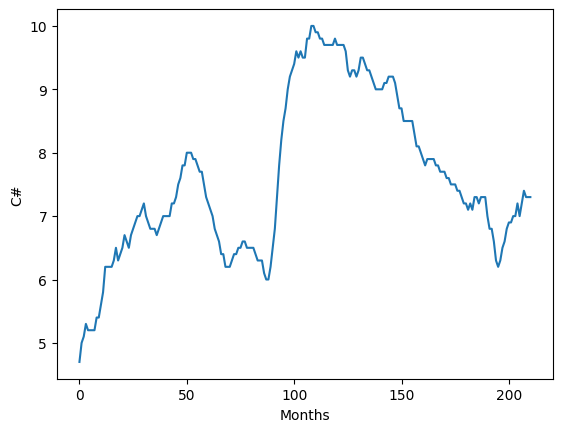
\includegraphics[scale=0.4]{lineplot/c-sharp.png}
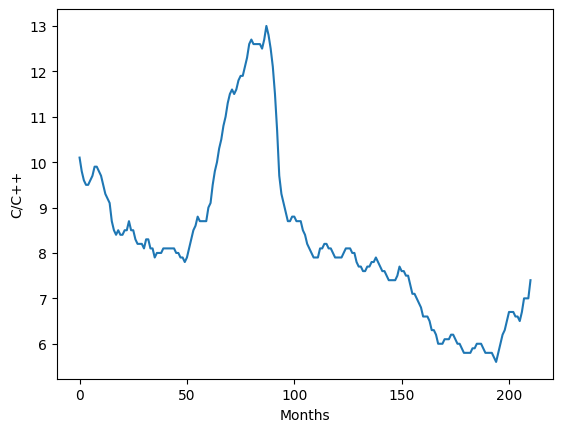
\includegraphics[scale=0.4]{lineplot/ccpp.png}

\subsection{\textit{Gaining Popularity}}
This category includes languages that are early in development and are gaining market rapidly.
These languages haven't been around for the entirety of the data set so due to the evident lack of data we cannot objectively conclude as per the quality and likeability of the language. For example Typescript is a rather young language, has a vibrant community and positive user growth.

\begin{itemize}
\item{Typescript}
\item{R}
\item{Groovy}
\item{Go}
\item{Dart}:At the peak of success, Dart controlled the market share of \(0.7%\) although it is not a market-dominant position by any stretch one can find a very high positive correlation \(0.901937\) with Python. 
\end{itemize}

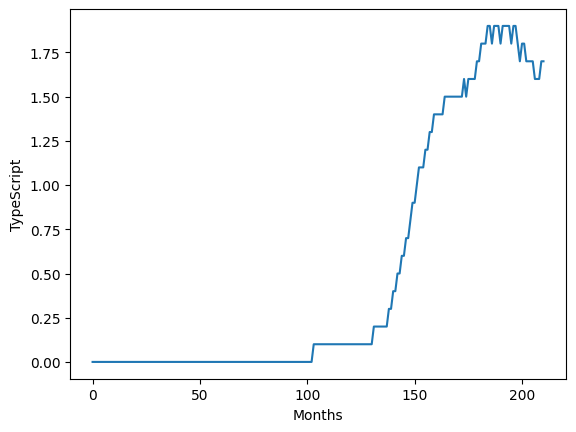
\includegraphics[scale=0.4]{lineplot/typescript.png}
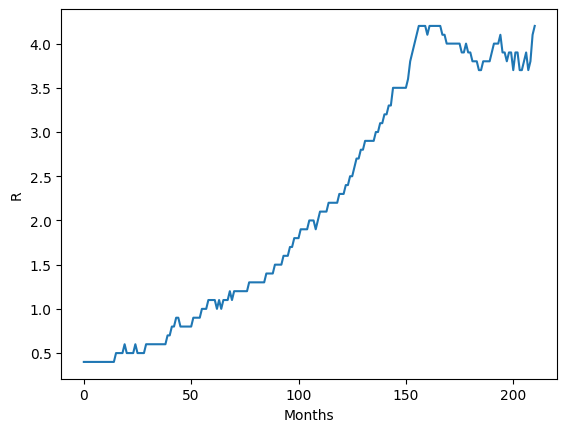
\includegraphics[scale=0.4]{lineplot/r.png}
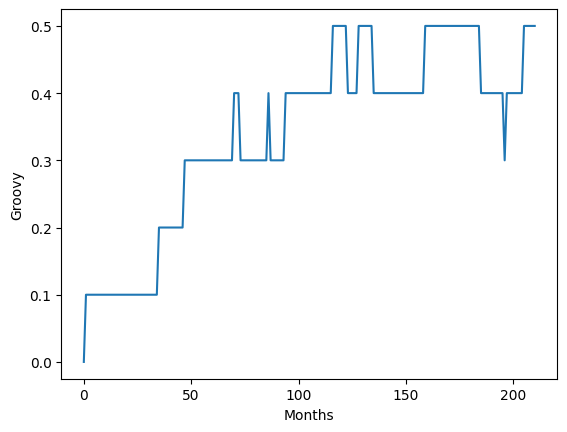
\includegraphics[scale=0.4]{lineplot/groovy.png}
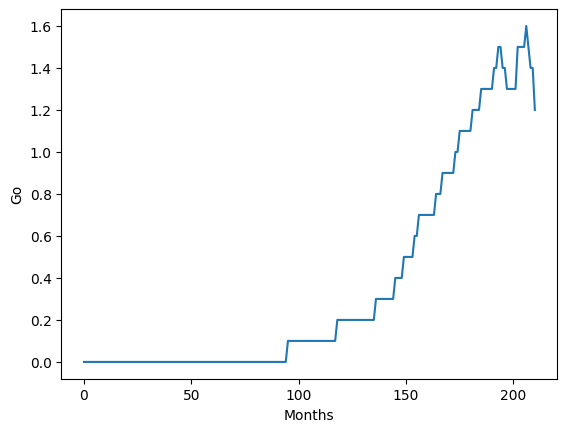
\includegraphics[scale=0.4]{lineplot/go.png}
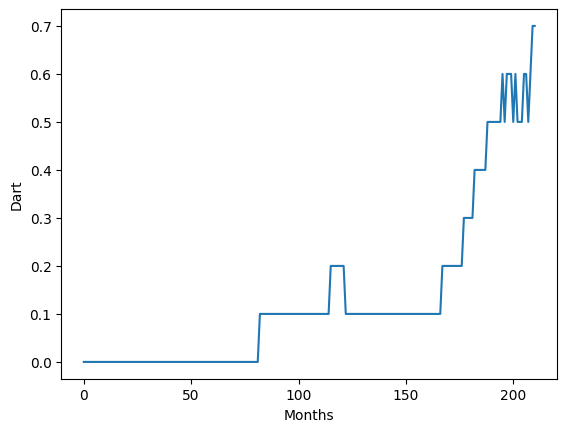
\includegraphics[scale=0.4]{lineplot/dart.png}

\subsection{Correlation}
In statistics, correlation or dependence is any statistical relationship, whether causal or not, between two random variables or bivariate data. Although in the broadest sense, "correlation" may indicate any type of association, in statistics it usually refers to the degree to which a pair of variables are linearly related. Familiar examples of dependent phenomena include the correlation between the height of parents and their offspring, and the correlation between the price of a good and the quantity the consumers are willing to purchase, as it is depicted in the so-called demand curve.

Correlations are useful because they can indicate a predictive relationship that can be exploited in practice. For example, an electrical utility may produce less power on a mild day based on the correlation between electricity demand and weather. In this example, there is a causal relationship, because extreme weather causes people to use more electricity for heating or cooling. However, in general, the presence of a correlation is not sufficient to infer the presence of a causal relationship (i.e., correlation does not imply causation). 

In our analysis we have found that Java was the top language till April 2018, starting from July 2004. Then the top spot has been reserved by Python, till the end of our sample size. Seeing this we decided to run a comprehensive analysis of the correlation between python and Java. We have also included their correlation to other languages.

\subsection{Correlation between other languages and Python and Java}
\begin{center}
\begin{tabular}{ c c c }
Languages & Python & Java\\\\

Abap & 0.210543 & -0.275354\\
Ada & 0.677052 & -0.711266\\
C/C++ & -0.702704 & 0.681450\\
C-Sharp & 0.085039 & -0.169606\\
Cobol & -0.514747 & 0.534975\\
Dart & 0.901937 & -0.891201\\
Delphi/Pascal & -0.803821 & 0.842192\\
Go & 0.985374 & -0.957954\\
Groovy & 0.676539 & -0.719915\\
Haskell & 0.028710 & -0.049515\\
Java & -0.983492 & 1.000000\\
Javascript & 0.385331 & -0.322988\\
Julia & 0.905960 & -0.939636\\
Kotlin & 0.945595 & -0.892701\\
Lua & 0.069608 & -0.154700\\
Matlab & -0.617304 & 0.529346\\
Objective-C & 0.325187 & -0.431106\\
Perl & -0.783993 & 0.826646\\
PHP & -0.943219 & 0.966258\\
Python & 1.000000 & -0.983492\\
R & 0.900140 & -0.933396\\
Ruby & -0.441982 & 0.411585\\
Rust & 0.925995 & -0.916171\\
Scala & 0.733003 & -0.777016\\
Swift & 0.695197 & -0.745004\\
Typescript & 0.970837 & -0.944515\\
VBA & -0.602485 & 0.588156\\
Visual Basic & -0.870000 & 0.898426\\

\end{tabular}
\end{center}

\subsection{Correlation between the rise and fall of Python and Java}

\begin{lstlisting}
import numpy as np
import pandas as pd
import seaborn as sb

data = pd.read_csv('data/original_data.csv');
data.to_csv('data/ad3.csv', float_format='%.3f')

sb.regplot(x='Python', y='Java', data = data)
data2 = data.drop(columns = ['Months','Date'])

corelation = data2.corr()
corelation[['Python', 'Java']]

data3 = data[['Months', 'Python', 'Java']]
data3 = data3.set_index('Months')

sb.lineplot(data = data3)
\end{lstlisting}

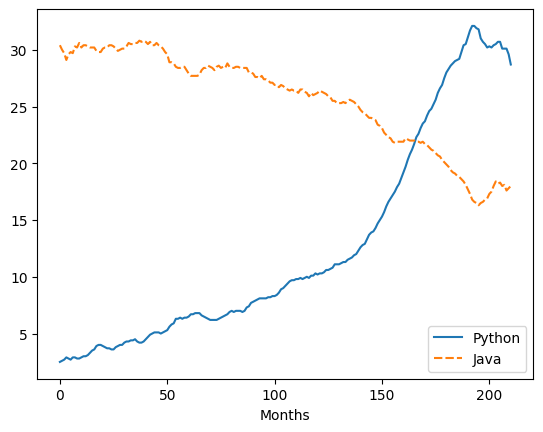
\includegraphics[scale=0.5]{lineplot/java-v-python.png}\\
\texttt{A visual representation of the co-relation between Java and Python's fall and rise}\\

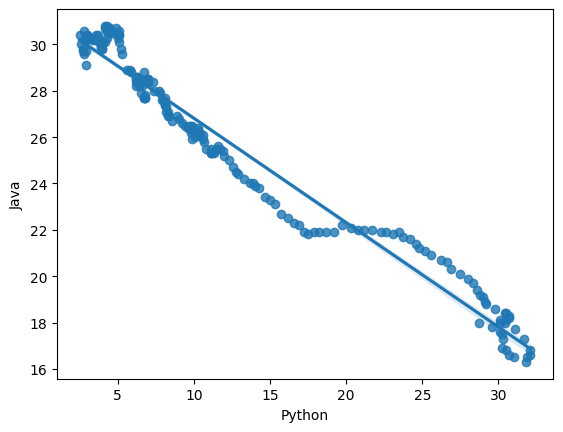
\includegraphics[scale=0.5]{regplot/java-v-python.png}\\
\texttt{A visual representation of the co-relation between Java and Python's fall and rise}

\section{Data}

\subsection{Data and derivatives}

\begin{itemize}
\item \href{https://github.com/0thorderlogic/smalldata/blob/main/data/backup.csv}{Original Data CSV file}
\item \href{https://github.com/0thorderlogic/smalldata/tree/main/barplot}{Barplot graphs of all langauages}
\item \href{https://github.com/0thorderlogic/smalldata/tree/main/lineplot}{Lineplot graphs of all langauages}
\item \href{https://github.com/0thorderlogic/smalldata/tree/main/regplot}{Regplot graphs of all langauages}
\end{itemize}

\subsection{Jupyter Notebook}

\begin{itemize}
\item \href{https://github.com/0thorderlogic/smalldata/blob/main/main.ipynb}{Main}
\item \href{https://github.com/0thorderlogic/smalldata/blob/main/correlation.ipynb}{Correlation}
\item \href{https://github.com/0thorderlogic/smalldata/blob/main/visuals.ipynb}{Visualisation}
\end{itemize}


\section{Acknowledgment}

The whole team would like to attribute the successful completion of this project to our friends and the internet at large.

\section*{}

\begin{thebibliography}{00}
\bibitem{b1}Correlation (2023) Wikipedia. Available at: https://en.wikipedia.org/wiki/Correlation (Accessed: 20 July 2023). 

\bibitem{b2}@article{Waskom2021,
    doi = {10.21105/joss.03021},
    url = {https://doi.org/10.21105/joss.03021},
    year = {2021},
    publisher = {The Open Journal},
    volume = {6},
    number = {60},
    pages = {3021},
    author = {Michael L. Waskom},
    title = {seaborn: statistical data visualization},
    journal = {Journal of Open Source Software}
 }
 \bibitem{b3}@Article{Hunter:2007,
  Author    = {Hunter, J. D.},
  Title     = {Matplotlib: A 2D graphics environment},
  Journal   = {Computing in Science \& Engineering},
  Volume    = {9},
  Number    = {3},
  Pages     = {90--95},
  abstract  = {Matplotlib is a 2D graphics package used for Python for
  application development, interactive scripting, and publication-quality
  image generation across user interfaces and operating systems.},
  publisher = {IEEE COMPUTER SOC},
  doi       = {10.1109/MCSE.2007.55},
  year      = 2007
}
\bibitem{b4}@software{reback2020pandas,
    author       = {The pandas development team},
    title        = {pandas-dev/pandas: Pandas},
    month        = feb,
    year         = 2020,
    publisher    = {Zenodo},
    version      = {latest},
    doi          = {10.5281/zenodo.3509134},
    url          = {https://doi.org/10.5281/zenodo.3509134}
}
\bibitem{b5}@InProceedings{ mckinney-proc-scipy-2010,
  author    = { {W}es {M}c{K}inney },
  title     = { {D}ata {S}tructures for {S}tatistical {C}omputing in {P}ython },
  booktitle = { {P}roceedings of the 9th {P}ython in {S}cience {C}onference },
  pages     = { 56 - 61 },
  year      = { 2010 },
  editor    = { {S}t\'efan van der {W}alt and {J}arrod {M}illman },
  doi       = { 10.25080/Majora-92bf1922-00a }
}
\bibitem{b6}@conference{Kluyver2016jupyter,
Title = {Jupyter Notebooks -- a publishing format for reproducible computational workflows},
Author = {Thomas Kluyver and Benjamin Ragan-Kelley and Fernando P{\'e}rez and Brian Granger and Matthias Bussonnier and Jonathan Frederic and Kyle Kelley and Jessica Hamrick and Jason Grout and Sylvain Corlay and Paul Ivanov and Dami{\'a}n Avila and Safia Abdalla and Carol Willing},
Booktitle = {Positioning and Power in Academic Publishing: Players, Agents and Agendas},
Editor = {F. Loizides and B. Schmidt},
Organization = {IOS Press},
Pages = {87 - 90},
Year = {2016}
} 
\bibitem{b7}@book{statistical,
  title={Statistical Methods (Combined)},
  isbn={9781259081071},
  url={https://books.google.co.in/books?id=PU0oNBfhn5gC},
  publisher={Tata McGraw-Hill Education}
}
\end{thebibliography}

\end{document}